\documentclass[notitlepage]{article}
\usepackage[margin = 2.5cm]{geometry}
\usepackage[utf8]{inputenc}
\usepackage{graphicx, dcolumn}

\usepackage{booktabs}

\title{Assignment 10 - Analysis}
\author{Franziska Rogg}
\date{\today}

\begin{document}

\maketitle

\clearpage
\section{Introduction}

This analysis examines the relationship between corruption and economic development using cross-country data. I aim to compare a level - level  and a level-log specification to assess whether the effec of GDP per capita on corruption is linear or non-linear. 


% ---------------------------------------------------------
\section{Plot}
% ----------------------------------------------------------

Figure 1 shows that the relationship between GDP per capita and corruption is non-linear

\begin{figure*}[htb!]
  \centering
  
  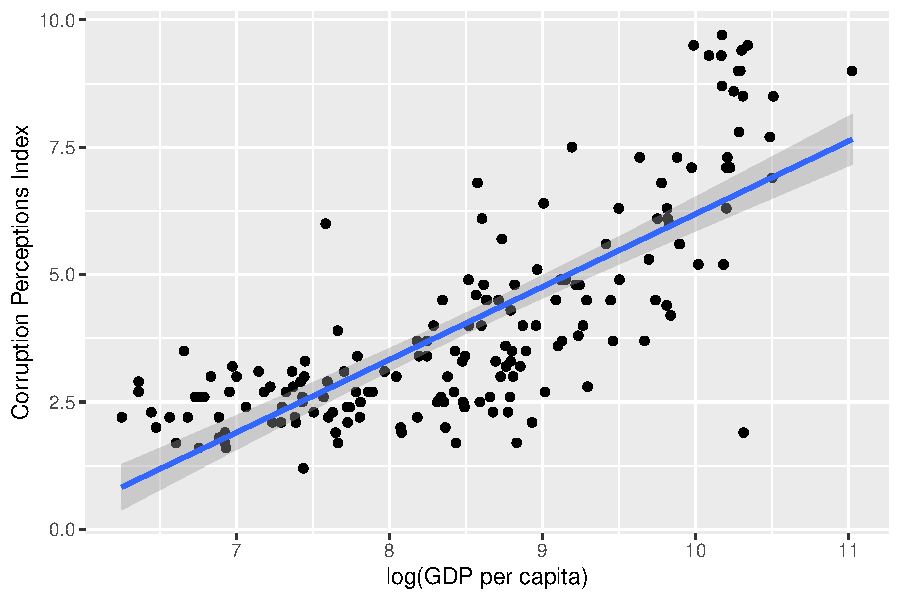
\includegraphics[width = 0.6\textwidth]{../graphs/scatter.pdf}
  \caption{GDP per capita and Corruption Perceptions Index}\label{fig1}
  
\end{figure*}

\clearpage

%----------------------------------------------------------
\section{Models}
% ----------------------------------------------------------

Table 1 compares the level-level model with the level-log model. When comparing the R2 values, it can be seen that the level-log model is the better fit for capturing this relationship. 

\begin{figure}[htb!] %---usually would be \begin{table} for tex tables
  \centering
  
  %------ THIS DOES NOT WORK FOR ME: \begin{table}
\centering
\begin{tabular}[t]{lcc}
\toprule
  & Level-Level & Level-Log\\
\midrule
(Intercept) & \num{2.502}*** & \num{-8.114}***\\
 & (\num{0.146}) & (\num{0.840})\\
undp\_gdp & \num{0.000}*** & \\
 & (\num{0.000}) & \\
log(undp\_gdp) &  & \num{1.431}***\\
 &  & (\num{0.104})\\
\midrule
R2 & \num{0.673} & \num{0.603}\\
Num.Obs. & \num{170} & \num{170}\\
\bottomrule
\multicolumn{3}{l}{\rule{0pt}{1em}+ p $<$ 0.1, * p $<$ 0.05, ** p $<$ 0.01, *** p $<$ 0.001}\\
\end{tabular}
\end{table}

  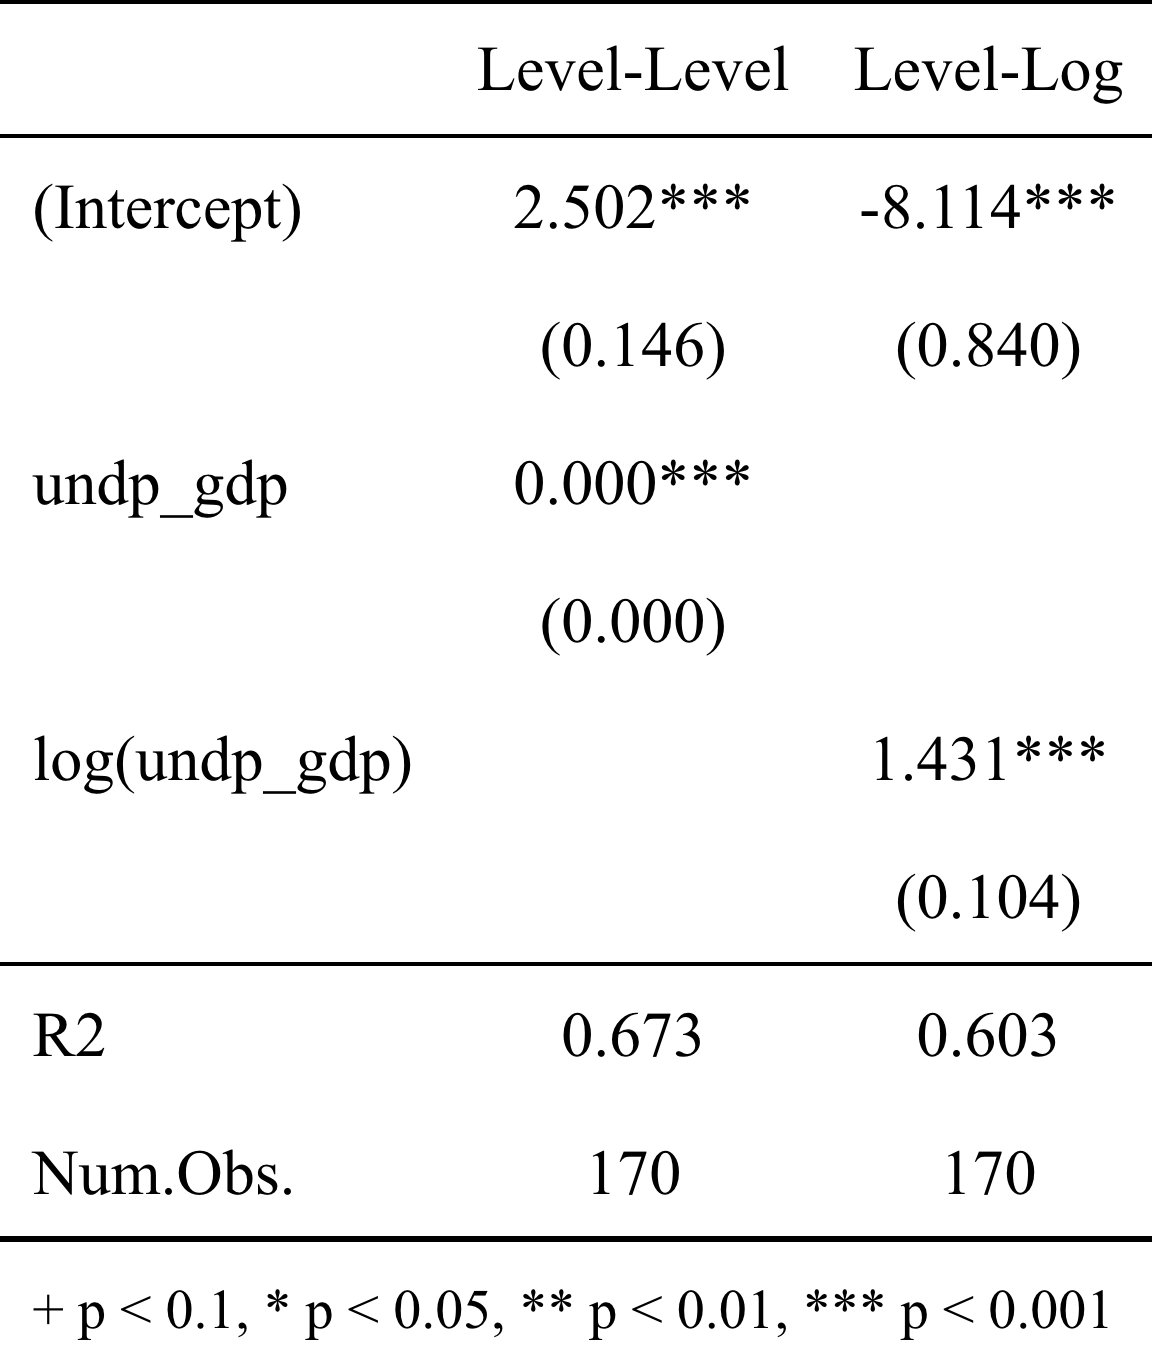
\includegraphics[width = 0.4\textwidth]{../tables/regression_table.png}
  \caption{Effect of (Log) GDP per capita on Corruption}\label{tab1}
\end{figure}


\end{document}





